% This file was created by tikzplotlib v0.9.2.
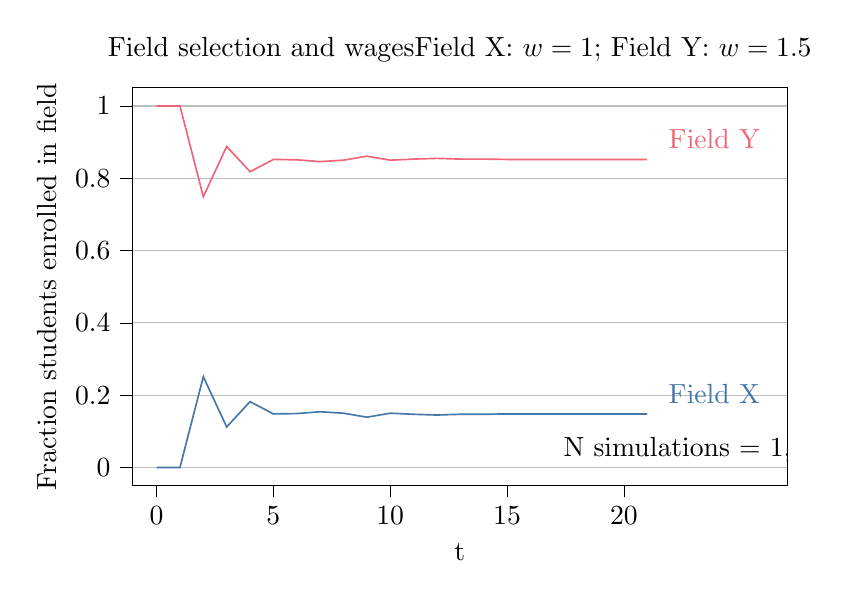
\begin{tikzpicture}

\definecolor{color0}{rgb}{0.266666666666667,0.466666666666667,0.666666666666667}
\definecolor{color1}{rgb}{0.933333333333333,0.4,0.466666666666667}

\begin{axis}[
height=6.6314113761540705cm,
tick align=outside,
tick pos=left,
title={Field selection and wages  \\ Field X: \(\displaystyle w = 1\); Field Y: \(\displaystyle w = 1.5\)},
width=9.904475999999999cm,
x grid style={white!69.0196078431373!black},
xlabel={t},
xmin=-1.05, xmax=27,
xtick style={color=black},
xtick={0,5,10,15,20},
xticklabels={\(\displaystyle 0\),\(\displaystyle 5\),\(\displaystyle 10\),\(\displaystyle 15\),\(\displaystyle 20\)},
ylabel={Fraction students enrolled in field},
ymajorgrids,
ymin=-0.05, ymax=1.05,
ytick style={color=black},
ytick={0,0.2,0.4,0.6,0.8,1},
yticklabels={\(\displaystyle 0\),\(\displaystyle 0.2\),\(\displaystyle 0.4\),\(\displaystyle 0.6\),\(\displaystyle 0.8\),\(\displaystyle 1\)}
]
\addplot [semithick, color0]
table {%
0 0
1 0
2 0.250999927520752
3 0.111999988555908
4 0.182000041007996
5 0.148000001907349
6 0.14900004863739
7 0.154000043869019
8 0.149999976158142
9 0.138999938964844
10 0.149999976158142
11 0.146999955177307
12 0.144999980926514
13 0.146999955177307
14 0.146999955177307
15 0.148000001907349
21 0.148000001907349
};
\addplot [semithick, color1]
table {%
0 1
1 1
2 0.749000072479248
3 0.888000011444092
4 0.818000078201294
5 0.851999998092651
6 0.851000070571899
7 0.845999956130981
8 0.850000023841858
9 0.861000061035156
10 0.850000023841858
11 0.852999925613403
12 0.855000019073486
13 0.852999925613403
14 0.852999925613403
15 0.851999998092651
21 0.851999998092651
};
\draw (axis cs:21.5,0.178) node[
  anchor=base west,
  text=color0,
  rotate=0.0
]{Field X};
\draw (axis cs:21.5,0.882) node[
  anchor=base west,
  text=color1,
  rotate=0.0
]{Field Y};
\draw (axis cs:17,0.03) node[
  anchor=base west,
  text=black,
  rotate=0.0
]{N simulations = 1,000};
\end{axis}

\end{tikzpicture}
